\setcounter{footnote}{0}
\renewcommand{\thefootnote}{[\roman{footnote}]} % for distinct numbering of Persian edition (chapter vi) footnotes (starting at [i])
\setlength{\footnotesep}{\baselineskip} % for space between footnotes
\tfarsi{%
\te{$\rceil$}\tfarsib{باب ششم}\te{\reversemarginpar\marginnote{{\footnotesize f.\thinspace 21b:\thinspace 20~\SjA,}~$\rceil$\\
{\footnotesize f.\thinspace 16a:\thinspace 25~\SjB\phantom{nn}}}}\\
در معرفت بعد كواكب از معدّل النهار.\hfill}
\\[0.5\baselineskip]

\noindent\normalmarginpar\marginnote{\hypertarget{Ppass1}{[1]}}
\tfarsi{%
عرض کوکب و میل ثاني درجه او، %
اگر هر دو در یک جهت باشند
جمع کنیم والا تفاضل بگیریم  و آن را حصّه بعد خوانیم  و جهت حصّه بعد
جهت مجموع یا جهت فضل باشد.\hfill}
\medskip

\noindent\normalmarginpar\marginnote{\hypertarget{Ppass2}{[2]}}\label{folio_break_persian_example}
\tfarsi{%
پس جيب حصّه بعد را در جیب تمام
میل منکوس درجه كوكب منحطّ ضرب کنیم حاصل جيب % 
\te{$\rceil$}%
بعد %
\te{\reversemarginpar\marginnote{{\footnotesize f.\thinspace 22a:\thinspace 1~\SjA}~$\rceil$}}%
بود.\hfill}
\\[\baselineskip]

\noindent\normalmarginpar\marginnote{\hypertarget{Ppass3}{[3]}}
\tfarsi{%
بوجهی\te{\footnote{ %
\tfarsi{بوجهی}~{$\Big ]$}~%
\raisebox{-.6ex}{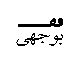
\includegraphics[scale=.85]{Images/qif_over_text_logograph.eps}}~\SjA. The overlining `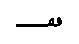
\includegraphics[scale=0.85]{Images/qif_arabic_logograph.eps}' over the word \tfarsi{بوجهی} is used to indicate a notable pause in the reading. As \textcite[173]{Gacek} explains, it is most likely a logograph (word-symbol) of the Arabic word \tfarsi{قف} (\qif) `stop' to indicate a pause in reading; or alternatively, the abbreviation \tfarsi{فتــ‬} (\textit{fata--}) of the phrase \tfarsi{فتأملها} (\fatammalha)
`reflect on it'.\label{qif_overlinning}}}
دیگر جيب حصّه بعد را در جیب تمام میل کلّی ضرب کنیم
و حاصل را بر جيب تمام میل\te{\footnote{ % 
\tfarsi{میل}~{$\Big ]$}~\tfarsi{%
میل \cancel{کلّی}}~\SjA, cancellation \textit{intra lineam}.}}
ثاني درجه آن کوکب قسمت کنیم
خارج  
\te{$\rceil$}%
قسمت %  
\te{\reversemarginpar\marginnote{{\footnotesize f.\thinspace 16b:\thinspace 1~\SjB}~$\rceil$}}%
جيب بعد باشد و جهت آن جهت حصّه بعد باشد.\hfill}
\medskip

\noindent\normalmarginpar\marginnote{\hypertarget{Ppass4}{[4]}}
\tfarsi{%
و چون جيب حصّه بعد را در جدول جيب تمام میل کلّی درآرند و حاصل را بر جيب تمام میل ثاني درجه آن کوکب  قسمت کنند خارج قسمت جيب بعد باشد.\hfill}
\medskip

\noindent\normalmarginpar\marginnote{\hypertarget{Ppass5}{[5]}}
\tfarsi{%
و اگر کوکب را عرض نباشد، میل درجه او بعد باشد.\hfill}

%%%%%%%%%%%%%%%%%%%%%%%%%%%%%%%%%
\clearpage\phantomsection
%%%%%%%%%%%%%%%%%%%%%%%%%%%%%%%%%

\textbf{Sixth chapter} \\
On the \gls{knowledge} (\marifat) of the \glspl{distance_celestial_object} (\bud\idafaconsonant\ \kawakib\ \az\ \muaddil\ \alnahar).   
\\[0.5\baselineskip]

\noindent\reversemarginpar\marginnote{\hypertarget{PEpass1}{[1]}}%
{[Given]} the \gls{latitude_celestial_object} (\ard\idafaconsonant\ \kawkab) and the \gls{second_declination_degree} (\mayl\idafaconsonant\ \thani\idafavowel\ \daraji\idafavowel\ \uy), if both should be in \gls{one_direction} (\yik\ \jahat), we \gls{sum} (*\jam\ \kardan) [them]; otherwise, we should take the \gls{difference} (\tafadul). And we call that [result] the \gls{share_of_distance} (\hissi\idafavowel\ \bud). And the \gls{direction_share_of_distance} (\jahat\idafaconsonant\ \hissi\idafavowel\ \bud) should be the \gls{direction_sum} (\jahat\idafaconsonant\ \majmu) or the \gls{direction_residue} (\jahat\idafaconsonant\ \fadla). 
\label{passage_1_english_persian} 
\medskip

\noindent\reversemarginpar\marginnote{\hypertarget{PEpass2}{[2]}}%
Then, we \glslink{low_multiplication}{low-multiply} (*\munhatt\idafaconsonant\ \darb\ \kardan) the \gls{Sine_share_of_distance} (\jayb\idafaconsonant\ \hissi\idafavowel\ \bud) in the \gls{Cosine_inverse_declination_degree_celestial_object} (\jayb\idafaconsonant\ \tamam\idafaconsonant\ \mayl\idafaconsonant\ \mankus\idafaconsonant\ \daraji\idafavowel\ \kawkab). The \gls{result} (\hasil) is the \gls{Sine_distance} (\jayb\idafaconsonant\ \bud). 
\\[\baselineskip]

\noindent\reversemarginpar\marginnote{\hypertarget{PEpass3}{[3]}}%
In another way, we \glslink{multiplication}{multiply} (*\darb\ \kardan) the \gls{Sine_share_of_distance} (\jayb\idafaconsonant\ \hissi\idafavowel\ \bud) in the \gls{Cosine_maximum_declination} (\jayb\idafaconsonant\ \tamam\idafaconsonant\ \mayl\idafaconsonant\ \kulli) [\ie  in the Cosine of the ecliptic obliquity] and we \glslink{division}{divide} (*\qismat\ \kardan) the \gls{result} (\hasil) over the \gls{Cosine_second_declination_degree} (\jayb\idafaconsonant\ \tamam\idafaconsonant\ \mayl\idafaconsonant\ \thani\idafavowel\ \daraji) of that \gls{celestial_object} (\kawkab). The \glslink{quotient_division}{quotient of the division} (\kharij\idafaconsonant\ \qismat) should be the \gls{Sine_distance} (\jayb\idafaconsonant\ \bud), and its \gls{direction} (\jahat)  should be the \gls{direction_share_of_distance} (\jahat\idafaconsonant\ \hissi\idafavowel\ \bud). 
\medskip

\noindent\reversemarginpar\marginnote{\hypertarget{PEpass4}{[4]}}%
And since they \gls{extract} (*\darardan) [the product of the multiplication with] the \gls{Sine_share_of_distance} (\jayb\idafaconsonant\ \hissi\idafavowel\ \bud) from the \gls{table_Cosine_maximum_declination} (\jadval\idafaconsonant\ \jayb\idafaconsonant\ \tamam\idafaconsonant\ \mayl\idafaconsonant\ \kulli) [\ie in the table of the Cosine of the ecliptic obliquity] and they \glslink{division}{divide} (*\qismat\ \kardan) the \gls{result} (\hasil) over the \gls{Cosine_second_declination_degree} (\jayb\idafaconsonant\ \tamam\idafaconsonant\ \mayl\idafaconsonant\ \thani\idafavowel\ \daraji) of that \gls{celestial_object} (\kawkab), the \glslink{quotient_division}{quotient of the division} (\kharij\idafaconsonant\ \qismat) should be the \gls{Sine_distance} (\jayb\idafaconsonant\ \bud).
\medskip

\noindent\reversemarginpar\marginnote{\hypertarget{PEpass5}{[5]}}%
And if a \gls{celestial_object} (\kawkab) should have no \gls{latitude} (\ard), the \gls{declination_degree} (\mayl\idafaconsonant\ \daraji\idafavowel\ \uy) should be the \gls{distance} (\bud). 

%%%%%%%%%%%%%%%%%%%%%%%%%%%%%%%%%
\clearpage\phantomsection
%%%%%%%%%%%%%%%%%%%%%%%%%%%%%%%%%

\noindent\normalmarginpar\marginnote{\hypertarget{Ppass6}{[6]}}
\tfarsi{%
و اگر عرض باشد اما درجه او را میل نباشد، جيب عرض او را در جیب تمام میل كلّی منحطّ ضرب کنیم
یا در\te{\footnote{ %
\tfarsi{یا در}~{$\Big ]$}~%
\tfarsi{یاد در}~\SjB, dittography of the first \tfarsi{د}.\label{emeneded_attested_persian_example}}}   
جدول سابق درآریم
حاصل جيب بعد باشد و جهت او جهت عرض باشد.\hfill}
\medskip

\noindent\normalmarginpar\marginnote{\hypertarget{Ppass7}{[7]}}
\tfarsi{%
و اگر میل درجه او میل كلّی باشد، حصّة البعد بعينه بعد باشد.\hfill}
\\[\baselineskip]

\noindent\normalmarginpar\marginnote{\hypertarget{Ppass8}{[8]}}
\tfarsi{%
و بوجهی\te{\footnote{ %
\tfarsi{و بوجهی}~{$\Big ]$}~%
\raisebox{-.6ex}{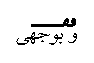
\includegraphics[scale=.85]{Images/qif_over_text_logograph_2.eps}}~\SjA, with emphasis. \Vid\ footnote~\ref{qif_overlinning}.}}
دیگر جيب بعد درجه کوکب از انقلاب اقرب در جیب
تمام عرض کوکب منحطّ ضرب کنیم حاصل جیب بعد کوکب از
دایرهٔ ماره باقطاب اربعه %
\wrapfootnote{%
باشد.\hfill\break
\te{\phantom{a}}\break % Required to allow a line break within a single \tfarsi{} group (Hack!)
\te{\noindent\normalmarginpar\marginnote{\hypertarget{Ppass9}{[9]}}}%
پس جیب عرض کوکب را بر جيب تمام بعد از دایرهٔ ماره باقطاب اربعه}%
{ %
\tfarsi{باقطاب اربعه}%
\thinspace\dots\thinspace
\tfarsi{باشد.\@  پس}~\te{$\Big ]$}
\begin{itemize}
    \item 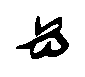
\includegraphics[height=.75em]{Images/marginal_insertion_end.eps}~~%
\tfarsi{باقطاب اربعه}%
\thinspace\dots\thinspace
\tfarsi{پس} %
$\stackrel{\text{\tiny\signederenvoi}}{\text{\tfarsi{باشد}}}$~\SjA, %
inserted in the exterior margin by the same hand.
The penultimate word of passage~[8] on f.\thinspace 22a:\thinspace 6  has 
an insertion mark `\signederenvoi' (\textit{signe-de-renvoi}) placed above it, \scl  \dots\thinspace\tfarsi{منحطّ} %
$\stackrel{\text{\tiny\signederenvoi}}{\text{\tfarsi{اربعه} }}$ %
\tfarsi{باقطاب}\thinspace\dots\thinspace .  
The first word of the marginal text also bears the same mark, \textit{supra verbum}, \scl\ \dots\thinspace
\tfarsi{پس} %
$\stackrel{\text{\tiny\signederenvoi}}{\text{\tfarsi{باشد}}}$. The marginal text ends with  `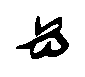
\includegraphics[height=.75em]{Images/marginal_insertion_end.eps}': this could be a calligraphic variant of the abbreviation \tfarsi{هى} (\textit{hā}\Ayn) of the Arabic word \tfarsi{إنتهى} (\intiha) meaning `it is finished', \vid\ \textcite[117]{Gacek};
\item \tfarsi{باقطاب اربعه}%
\thinspace\dots\thinspace
\tfarsi{باشد.\@  پس}~\textit{omitted} \SjB,  per homeoteleuton. The penultimate word \tfarsi{\underline{اربعه}} of passage~[8], %
before the missing text, is identical to the last word of the missing text %
\tfarsi{\underline{اربعه} منحطّ\thinspace\dots}\thinspace %
 in  passage~[9].\\[5pt]
\textbf{\scshape remark}: MS~Or.\thinspace 566 of the \ZijUlughBeg\ from  University Library (Cambridge) is also missing the same amount of text. The missing words \tfarsi{باشد\thinspace\dots\thinspace اربعه} span the length of a line between the end of line 18 (at \tfarsi{اربعه}) %
and the beginning of line 19 (at \tfarsi{منحطّ}) on folio 16r of this manuscript.\label{zij_ulugh_beg_missing_line}
\end{itemize}\vspace{-\topsep}
} %
منحطّ قسمت کنیم %
\wrapfootnote{و به خارج قسمت}%
{\tfarsi{%
و~به~خارج~قسمت
}~\te{$\Big ]$}~\tfarsi{
و به خارج قسمت کنیم  و به خارج قسمت
}~\SjB, dittography of the second \tfarsi{و به خارج قسمت}. %
I suspect a parableptic error as the word \tfarsi{قسمت} %
appears twice on the line in close proximity: 
\dots\thinspace \tfarsi{\underline{قسمت} از}\thinspace\dots\thinspace\tfarsi{\underline{قسمت} کنیم}\thinspace\dots\thinspace.\label{wrap_footnote_example}}
از جدول جيب قوس بگیریم و آن را قوس اوّل خوانیم  و جهت آن جهت عرض کوکب بود.\hfill}

%%%%%%%%%%%%%%%%%%%%%%%%%%%%%%%%%
\clearpage\phantomsection
%%%%%%%%%%%%%%%%%%%%%%%%%%%%%%%%%

\noindent\reversemarginpar\marginnote{\hypertarget{PEpass6}{[6]}}%
And if the \gls{latitude} (\ard) [of a celestial object] should exist but \gls{its_degree} (\daraji\idafavowel\ \uy)  should have no \gls{declination}  (\mayl), we  \glslink{low_multiplication}{low-multiply} (*\munhatt\idafaconsonant\ \darb\ \kardan) the \gls{Sine_latitude} (\jayb\idafaconsonant\ \ard\idafaconsonant\ \uy) in the \gls{Cosine_maximum_declination} (\jayb\idafaconsonant\ \tamam\idafaconsonant\ \mayl\idafaconsonant\ \kulli)  [\ie  in the Cosine of the ecliptic obliquity], or we \gls{extract} (*\darardan) [the product of this multiplication] from the preceding \gls{table} (\jadval) [\ie in the table of the Cosine of the maximum declination]. The \gls{result} (\hasil) should be the \gls{Sine_distance} (\jayb\idafaconsonant\ \bud), and its \gls{direction} (\jahat) should be the \gls{direction_latitude} (\jahat\idafaconsonant\ \ard).\label{passge_6_ard_glossary_format_example}
\medskip

\noindent\reversemarginpar\marginnote{\hypertarget{PEpass7}{[7]}}%
And if the \gls{declination_degree} (\mayl\idafaconsonant\ \daraji\idafavowel\ \uy) should be the \gls{maximum_declination} (\mayl\idafaconsonant\ \kulli) [\ie the obliquity of the ecliptic], the \gls{share_of_distance} (\hissatalbud) itself should be the \gls{distance} (\bud). 
\\[\baselineskip]

\noindent\reversemarginpar\marginnote{\hypertarget{PEpass8}{[8]}}%
And in another way, we \glslink{low_multiplication}{low-multiply} (*\munhatt\idafaconsonant\ \darb\ \kardan) the \gls{Sine_distance_celestial_object_nearest_solstice} (\jayb\idafaconsonant\ \bud\idafaconsonant\ \daraji\idafavowel\ \kawkab\ \az\ \inqilab\idafaconsonant\ \aqrab) in the \glsuseri{Cosine_latitude_celestial_object} (\jayb\idafaconsonant\ \tamam\idafaconsonant\ \ard\idafaconsonant\ \kawkab). The \gls{result} (\hasil) should be the
\glslink{Sine_distance_celestial_object_solstitial_colure}{Sine of the distance of the celestial object from the `circle passing through the four poles'} [\ie from the `solstitial colure'] (\jayb\idafaconsonant\ \bud\idafaconsonant\ \kawkab\ \az\ \guillemotleft\dayiri\idafavowel\ \marri\ \biaqtab\idafaconsonant\ \arbai\guillemotright). 
\medskip

\noindent\reversemarginpar\marginnote{\hypertarget{PEpass9}{[9]}}%
Then, we \glslink{low_division}{low-divide} (*\munhatt\idafaconsonant\ \qismat\ \kardan) the \gls{Sine_latitude_celestial_object} (\jayb\idafaconsonant\ \ard\idafaconsonant\ \kawkab) over the \glslink{Cosine_distance_solstitial_colure}{Cosine of the distance [of the celestial object] from the `circle passing through the four poles'} (\jayb\idafaconsonant\ \tamam\idafaconsonant\ \bud\ \az\ \guillemotleft\dayiri\idafavowel\ \marri\ \biaqtab\idafaconsonant\ \arbai\guillemotright). And for the \glslink{quotient_division}{quotient of the division} (\kharij\idafaconsonant\ \qismat), we should take the \gls{arc} (\qaws) from the \gls{table_of_Sine} (\jadval\idafaconsonant\ \jayb). And we call it the \gls{first_arc} (\qaws\idafaconsonant\ \avval) and its \gls{direction} (\jahat) is the \gls{direction_latitude_celestial_object} (\jahat\idafaconsonant\ \ard\idafaconsonant\ \kawkab). 

%%%%%%%%%%%%%%%%%%%%%%%%%%%%%%%%%
\clearpage\phantomsection
%%%%%%%%%%%%%%%%%%%%%%%%%%%%%%%%%

\noindent\normalmarginpar\marginnote{\hypertarget{Ppass10}{[10]}}
\tfarsi{%
پس اگر عرض و میل درجه كوكب هر دو در یک جهت باشند، قوس اوّل و میل كلّی را جمع کنیم. و اگر از 
ربع\te{\footnote{ %
\tfarsi{ربع}~{$\Big ]$}  
\begin{itemize}
    \item \tfarsi{بع}\cancel{\tfarsi{ا}}\tfarsi{ر}~\SjA,  erasure
\textit{intra lineam};
    \item \tfarsi{رابع}~\SjB. The Arabic words \tfarsi{ربع} (\rub) and \tfarsi{رابع} (\rabi) are the fractional (`one-fourth') and ordinal (`fourth') forms of the number four \tfarsi{أربعة} (\arbai) respectively. The mathematical context of the passage supports the fractional meaning `one-fourth' or a `quarter'. The reading in \SjB\ could be a semantic mistake by the scribe in copying Arabic loanwords (\muarrab).
\end{itemize}\vspace{-\topsep}}}
دور زیاده شود، تمام مجموع تا نصف دور بگیریم. و اگر در جهت مختلف باشند، تفاضل میان هر دو بگیریم حاصل قوس دوم باشد و جهتش جهت مجموع یا جهت فضل باشد.\hfill}
\medskip

\noindent\normalmarginpar\marginnote{\hypertarget{Ppass11}{[11]}}
\tfarsi{%
پس جیب قوس دوم را در جیب تمام بعد از
دایرهٔ ماره باقطاب اربعه منحطّ ضرب کنیم حاصل جيب بعد کوکب باشد  و جهتش جهت قوس دوم باشد.\hfill}

%%%%%%%%%%%%%%%%%%%%%%%%%%%%%%%%%
\clearpage\phantomsection
%%%%%%%%%%%%%%%%%%%%%%%%%%%%%%%%%

\noindent\reversemarginpar\marginnote{\hypertarget{PEpass10}{[10]}}%
Then, if the \gls{latitude} (\ard) and the \gls{declination_degree_celestial_object} (\mayl\idafaconsonant\ \daraji\idafavowel\ \kawkab) both should be in \gls{one_direction} (\yik\ \jahat), we \gls{sum} (*\jam\ \kardan) the \gls{first_arc} (\qaws\idafaconsonant\ \avval) and the \gls{maximum_declination} (\mayl\idafaconsonant\ \kulli) [\ie the ecliptic obliquity]. And if [the sum] \gls{exceeds} (*\ziyadi\ \shudan) \gls{one_quarter} (\rabi) [\ie is greater than 90\degree], we should take the \gls{whole_sum} (\tamam\idafaconsonant\ \majmu) up to \gls{one_half} (\nisf) [\ie up to 180\degree]. And if they should be in \gls{different_directions} (\jahat\idafaconsonant\ \mukhtalif), we should take the \gls{difference} (\tafadul) between the two; the \gls{result} (\hasil) [in both cases] should be [called] 
the \gls{second_arc} (\qaws\idafaconsonant\ \duvum) and its \gls{direction} (\jahat) should be the \gls{direction_sum} (\jahat\idafaconsonant\ \majmu) or the \gls{direction_residue} (\jahat\idafaconsonant\ \fadla). 
\medskip

\noindent\reversemarginpar\marginnote{\hypertarget{PEpass11}{[11]}}%
Then, we \glslink{low_multiplication}{low-multiply} (*\munhatt\idafaconsonant\ \darb\ \kardan) the \gls{Sine_second_arc} (\jayb\idafaconsonant\ \qaws\idafaconsonant\ \duvum) in the \glslink{Cosine_distance_solstitial_colure}{Cosine of the distance [of a celestial object] from the `circle passing through the four poles'} (\jayb\idafaconsonant\ \tamam\idafaconsonant\ \bud\ \az\ \guillemotleft\dayiri\idafavowel\ \marri\ \biaqtab\idafaconsonant\ \arbai\guillemotright). The result should be the \gls{Sine_distance_celestial_object} (\jayb\idafaconsonant\ \bud\idafaconsonant\ \kawkab) and its \gls{direction} (\jahat) should be the \gls{direction_second_arc}  (\jahat\idafaconsonant\ \qaws\idafaconsonant\ \duvum). 

%%%%%%%%%%%%%%%%%%%%%%%%%%%%%%%%%%%%%%%%%%%%%%%%%%%%%%%%%%%%%%%%%
